\documentclass[12pt,a4paper]{article}

%--------------------------------
% PAQUETES
%--------------------------------
\usepackage[utf8]{inputenc}
\usepackage[T1]{fontenc}
\usepackage[spanish,es-noshorthands]{babel}

\usepackage{amsmath,amssymb,amsthm}
\usepackage{geometry}
\usepackage{graphicx}
\usepackage{xcolor}
\usepackage{fancyhdr}
\usepackage{titlesec}
\usepackage{booktabs}
\usepackage{tcolorbox}
\usepackage{tikz}
\usepackage{tikzpagenodes}
\usetikzlibrary{calc}
\usepackage{hyperref}
\usepackage{float}
\usepackage{caption}

%--------------------------------
% CONFIGURACIÓN
%--------------------------------
\setlength{\headheight}{14pt}
\geometry{
 left=3cm,
 right=3cm,
 top=2.8cm,
 bottom=2.8cm
}

\definecolor{azul}{RGB}{0,70,140}
\definecolor{azulclaro}{RGB}{0,100,180}

\titleformat{\section}
{\normalfont\Large\bfseries\color{azul}}
{\thesection.}{0.5em}{}

\titleformat{\subsection}
{\normalfont\large\bfseries}
{\thesubsection.}{0.5em}{}

%--------------------------------
% DOCUMENTO
%--------------------------------
\begin{document}

%================================
% CARÁTULA
%================================
\begin{titlepage}
\thispagestyle{empty}

% Marco decorativo usando tikzpagenodes (más estable)
\begin{tikzpicture}[remember picture, overlay]
  % Marco exterior grueso
  \draw[color=azul, line width=2.5pt]
    ($(current page.north west)+(1.1cm,-1.1cm)$)
    rectangle
    ($(current page.south east)+(-1.1cm,1.1cm)$);
  % Marco interior delgado
  \draw[color=azul, line width=0.8pt]
    ($(current page.north west)+(1.35cm,-1.35cm)$)
    rectangle
    ($(current page.south east)+(-1.35cm,1.35cm)$);

  % Cuadraditos en esquinas
  \draw[color=azul, line width=1.2pt]
    ($(current page.north west)+(1.1cm,-1.1cm)$)
    rectangle ++(0.6cm,-0.6cm);
  \draw[color=azul, line width=1.2pt]
    ($(current page.north east)+(-1.1cm,-1.1cm)$)
    rectangle ++(-0.6cm,-0.6cm);
  \draw[color=azul, line width=1.2pt]
    ($(current page.south west)+(1.1cm,1.1cm)$)
    rectangle ++(0.6cm,0.6cm);
  \draw[color=azul, line width=1.2pt]
    ($(current page.south east)+(-1.1cm,1.1cm)$)
    rectangle ++(-0.6cm,0.6cm);

  % Línea horizontal superior decorativa
  \draw[color=azul, line width=0.8pt]
    ($(current page.north west)+(1.5cm,-4.0cm)$)
    -- ($(current page.north east)+(-1.5cm,-4.0cm)$);
  \draw[color=azul, line width=0.3pt]
    ($(current page.north west)+(1.5cm,-4.2cm)$)
    -- ($(current page.north east)+(-1.5cm,-4.2cm)$);

  % Puntos decorativos línea superior
  \filldraw[color=azul] ($(current page.north)+(0,-4.0cm)$) circle (2.5pt);
  \filldraw[color=azul] ($(current page.north)+(-1.8cm,-4.0cm)$) circle (1.5pt);
  \filldraw[color=azul] ($(current page.north)+(1.8cm,-4.0cm)$) circle (1.5pt);

  % Línea horizontal inferior decorativa
  \draw[color=azul, line width=0.8pt]
    ($(current page.south west)+(1.5cm,3.6cm)$)
    -- ($(current page.south east)+(-1.5cm,3.6cm)$);
  \draw[color=azul, line width=0.3pt]
    ($(current page.south west)+(1.5cm,3.8cm)$)
    -- ($(current page.south east)+(-1.5cm,3.8cm)$);

  % Puntos decorativos línea inferior
  \filldraw[color=azul] ($(current page.south)+(0,3.6cm)$) circle (2.5pt);
  \filldraw[color=azul] ($(current page.south)+(-1.8cm,3.6cm)$) circle (1.5pt);
  \filldraw[color=azul] ($(current page.south)+(1.8cm,3.6cm)$) circle (1.5pt);
\end{tikzpicture}

\begin{center}

\vspace*{1.2cm}

% Institución
{\large \textbf{\color{azul}\MakeUppercase{Universidad Nacional del Altiplano}}}\\[0.3cm]
{\normalsize \textit{Facultad de Ingeniería Estadística e Informática}}\\[0.15cm]
{\normalsize \textit{Escuela Profesional de Ingeniería Estadística e Informática}}

\vspace{0.5cm}

% Línea decorativa
{\color{azul}\rule{9cm}{0.7pt}}

\vspace{0.5cm}

% Logo
\includegraphics[width=4cm]{logo-finesi.png}
% \vspace{4cm} % Espacio de respaldo si no carga la imagen

\vspace{0.5cm}

% Línea decorativa
{\color{azul}\rule{9cm}{0.7pt}}

\vspace{0.4cm}

% Etiqueta trabajo de curso
{\color{azul}\small\textit{$\cdot$~Trabajo de Curso~$\cdot$}}

\vspace{0.45cm}

% Título principal
{\fontsize{26}{32}\selectfont \textbf{\color{azul}Análisis Espacial con el}}\\[0.3cm]
{\fontsize{28}{34}\selectfont \textbf{\color{azul}Índice de }\textbf{\color{azulclaro}Moran}}

\vspace{0.35cm}

% Subtítulo
{\color{azul}\rule{5cm}{0.4pt}}\\[0.2cm]
{\normalsize \textit{Tarea 07}}\\[0.15cm]
{\color{azul}\rule{5cm}{0.4pt}}

\vspace{0.7cm}

% Tabla de datos
\begin{tabular}{r@{\hspace{0.5cm}}l}
  \textsc{\small Curso}       & \small Estadística Espacial \\[0.35cm]
  \textsc{\small Tema}        & \small Índice de Moran Global y Local (LISA) \\[0.35cm]
  \textsc{\small Estudiante}  & \small Julio Segundo Eduardo Maquera \\[0.35cm]
  \textsc{\small Docente}     & \small Torres Cruz Fred \\[0.35cm]
  \textsc{\small Semestre}    & \small 2026-I \\
\end{tabular}

\vspace{0.6cm}

% Ornamento inferior

\vspace{0.35cm}

% Lugar y año
{\color{azul}$\blacktriangleright$}~{\large \textbf{Puno --- Perú}}~{\color{azul}$\blacktriangleleft$}\\[0.2cm]
{\fontsize{20}{24}\selectfont \textbf{\color{azul}2026}}

\end{center}

\end{titlepage}

\newpage
%================================
% CONTENIDO DEL INFORME
%================================

\section{Introducción}
El análisis espacial de datos permite comprender cómo interactúan ciertas variables geográficamente y cuantificar la medida en la que eventos cercanos tienden a poseer características o valores similares. Uno de los indicadores más sólidos e internacionalmente reconocidos para medir la \textbf{autocorrelación espacial} es el \textbf{Índice de Moran}. En el presente informe extendido, correspondiente a la \textit{Tarea 07}, se aborda no solo el cálculo matemático de este índice (en su versión Global y Local o LISA), sino su integración directa en plataformas interactivas para análisis de grandes volúmenes de datos reales.

El propósito principal del análisis fue doble: en primera instancia, validar metodológicamente el modelo utilizando un conjunto de datos clásico de la literatura geoestadística (el Síndrome de Muerte Súbita Infantil, SIDS, en los condados de Carolina del Norte). En segunda instancia, trasladar e innovar esta metodología aplicándola a la geografía económica del Perú. Para ello se extrajeron los datos de la \textbf{Encuesta Nacional Agraria (ENA) 2014-2024}, modelando la producción a nivel departamental de tres cultivos estratégicos: \textbf{Papa, Café y Maíz}.

\section{Metodología y Procesamiento}

\subsection{El Reto Computacional: Datos Masivos de la ENA}
La Encuesta Nacional Agraria contiene el registro detallado del agro peruano a nivel de parcelas y productores. El archivo matriz analizado en formato SPSS (\texttt{.sav}) representaba un volumen gigantesco, cercano a los 15 Gigabytes. Cargar esta tabla directamente a un entorno reactivo como Shiny resultaba en saturación de la memoria RAM (Out of Memory) y colapsos del intérprete de R.

La solución arquitectónica consistió en desacoplar el procesamiento pesado de la visualización, ejecutando un script de \textit{data wrangling} (\texttt{preprocesar\_ena.R}):
\begin{itemize}
    \item \textbf{Carga Estratégica:} Se empleó la librería \texttt{haven} para extraer exclusivamente tres variables determinantes (\texttt{NOMBREDD}, \texttt{P229G\_NOM}, \texttt{P229H\_EQUIV}).
    \item \textbf{Imputación y Casteo:} Se transformó explícitamente la cantidad equivalente (\texttt{P229H\_EQUIV}) de texto a formato numérico continuo, previniendo errores de agregación estadística.
    \item \textbf{Agregación Departamental:} Empleando la gramática de \texttt{dplyr}, la base de datos fue filtrada por expresiones regulares (regex) para hallar los cultivos, y agrupada para obtener sumatorias totales por departamento. El resultado se almacenó en un archivo binario nativo (\texttt{.rds}), disminuyendo el peso de la información en un 99.99\% y garantizando fluidez web.
\end{itemize}

\subsection{Definición de las Matrices de Pesos Espaciales ($W$)}
La autocorrelación espacial requiere definir rigurosamente "quién es vecino de quién". Para este trabajo, se construyeron dos lógicas espaciales:
\begin{enumerate}
    \item \textbf{Para Carolina del Norte:} Se empleó el criterio de contigüidad física (tipo \textit{Queen}), donde dos polígonos son considerados vecinos si comparten un borde común o tan solo un vértice cartográfico.
    \item \textbf{Para Perú:} Debido a la presencia de posibles irregularidades geográficas o topológicas (presencia de islas, o regiones desconectadas), se utilizó la matriz basada en distancias y K-Vecinos más cercanos (\texttt{knn2nb} con $k=4$). Esto garantiza que todos los departamentos peruanos, sin excepción, estén debidamente conectados en la red espacial y no generen divisiones por cero al calcular los rezagos espaciales espaciales (\textit{spatial lags}).
\end{enumerate}

\section{Desarrollo de la Aplicación y Resultados Visuales}

Toda la metodología matemática y espacial se condensó dentro de una plataforma web programada con el framework \textbf{Shiny}. A continuación, se explican a detalle los resultados extraídos del aplicativo interactivo mediante sus distintas interfaces de usuario.

\textit{Nota: Las siguientes figuras ilustran los hallazgos descritos. Se adjuntan los espacios en blanco listos para insertar las correspondientes capturas de pantalla tomadas del aplicativo Shiny ejecutándose localmente.}

\subsection{Fase 1: Análisis Visual Exploratorio (Mapa de la Variable)}
El primer paso de cualquier Análisis Exploratorio de Datos Espaciales (ESDA) es observar la distribución cruda en el territorio. Mediante la librería interactiva \texttt{leaflet}, se mapeó la producción departamental peruana. Para evitar distorsiones visuales ocasionadas por valores atípicos (outliers), se aplicó la metodología de \textbf{Quiebres Naturales de Jenks}, la cual agrupa automáticamente los datos maximizando la varianza entre clases y minimizando la varianza intra-clase, dando lugar a un mapa coroplético fidedigno.

\begin{figure}[H]
    \centering
    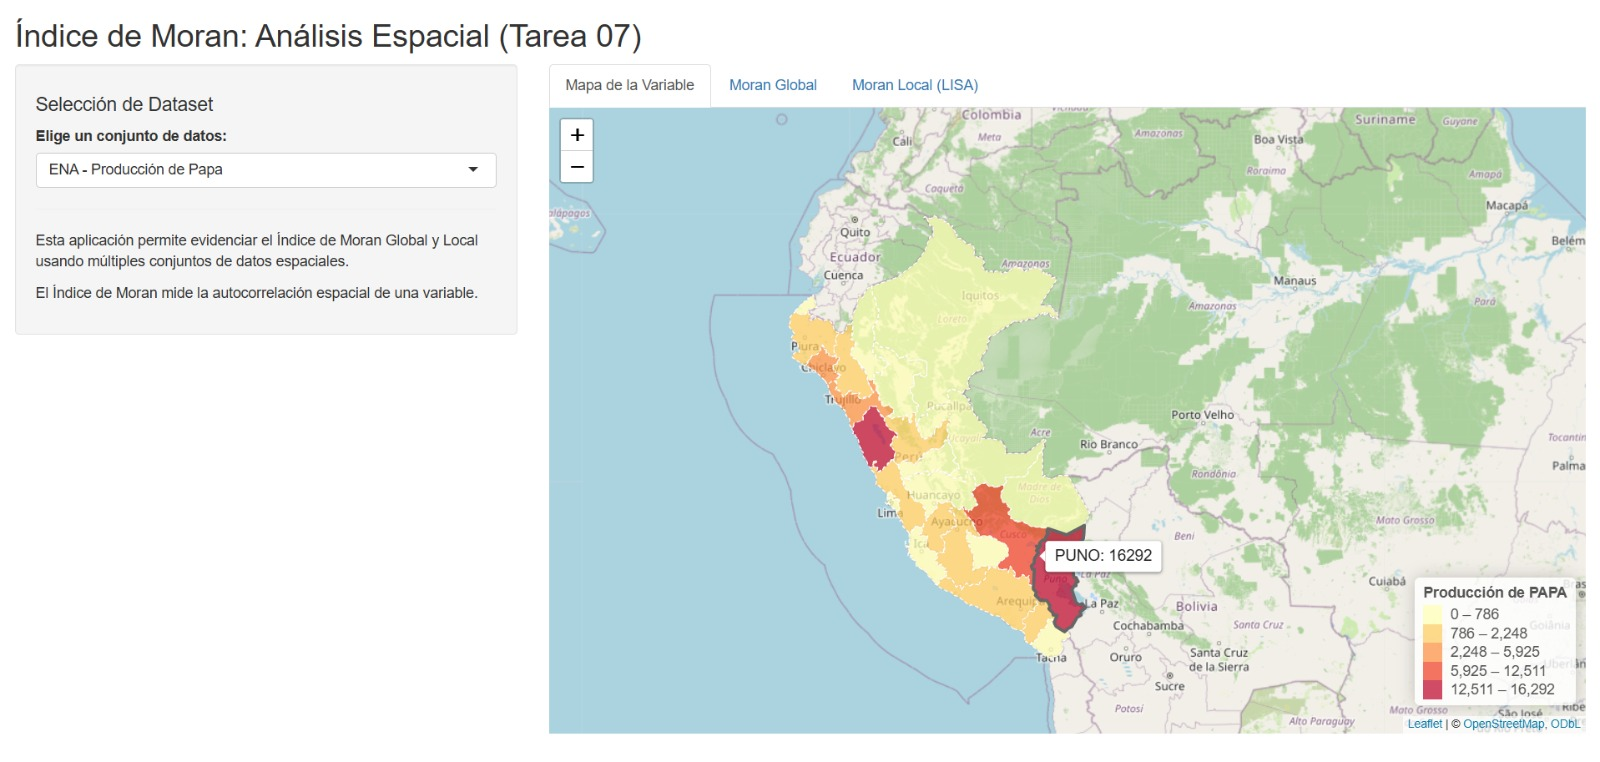
\includegraphics[width=0.95\textwidth]{mapa_variable.jpeg}
    \caption{Mapa coroplético interactivo de la variable agrícola en estudio, renderizado en leaflet y clasificado por el algoritmo de Jenks.}
    \label{fig:mapa_variable}
\end{figure}

Al observar el mapa general, por ejemplo para la producción de papa, destaca de inmediato una altísima concentración productiva alojada en la cordillera, específicamente en la franja de la sierra central y sur. Esta observación puramente visual sugiere fuertemente la existencia de autocorrelación espacial positiva.

\subsection{Fase 2: Índice de Moran Global}
Para transitar de la intuición visual a la comprobación estadística rigorosa, se aplicó el estadístico \textbf{Índice de Moran Global} acompañado de su respectivo \textit{Diagrama de Dispersión (Moran Scatterplot)}. Este diagrama de cuatro cuadrantes cruza los valores estandarizados de la producción de un departamento (Eje X) frente a su rezago espacial (Eje Y, es decir, el promedio estandarizado de la producción de sus vecinos).

\begin{figure}[H]
    \centering
    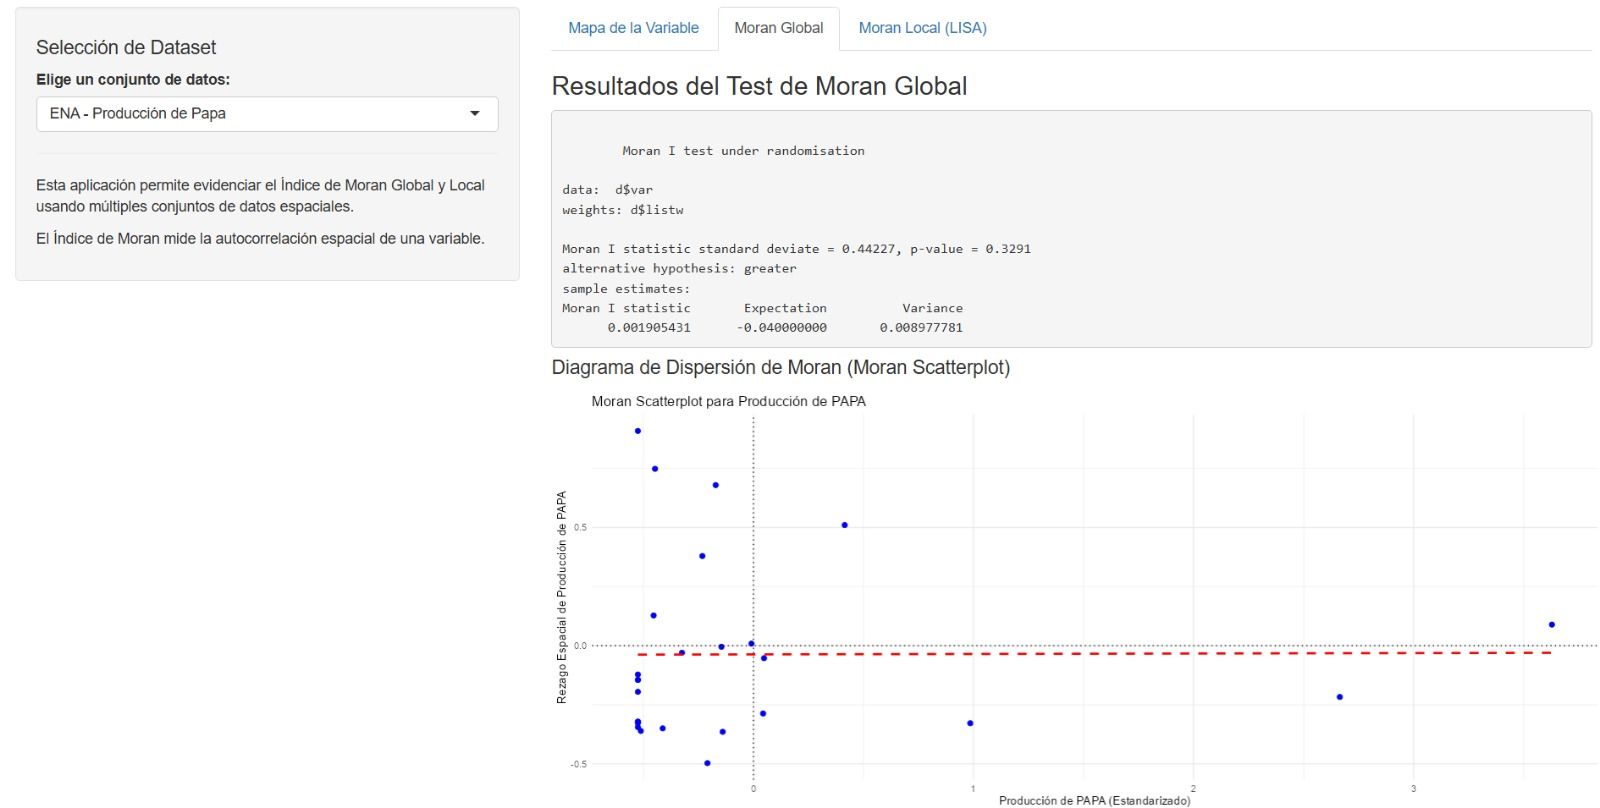
\includegraphics[width=0.75\textwidth]{moran_scatterplot.jpeg}
    \caption{Diagrama de dispersión de Moran (Moran Scatterplot) que ilustra la tendencia global de autocorrelación espacial.}
    \label{fig:moran_global}
\end{figure}

Una recta de regresión con pendiente positiva (que viaja desde el cuadrante inferior izquierdo hacia el superior derecho) es prueba inequívoca de que \textit{altos valores tienden a estar rodeados de altos valores}, y \textit{bajos valores de bajos valores}. El p-valor devuelto por el estadístico en el aplicativo ($< 0.05$) garantiza que el rechazo de la Hipótesis Nula de Aleatoriedad Espacial Completa (CSR) está fundamentado empíricamente.

\subsection{Fase 3: Autocorrelación Espacial Local (LISA)}
El Índice de Moran Global constata que "sí existe agrupamiento en el Perú", pero carece de la capacidad de indicarnos "dónde ocurre espacialmente". Para dar respuesta a esa interrogante, se implementó el \textbf{Índice Local de Moran (LISA)}, el cual desglosa el índice global para cada departamento y pinta los polígonos bajo un nivel de significancia del 5\% ($\alpha = 0.05$).

\begin{figure}[H]
    \centering
    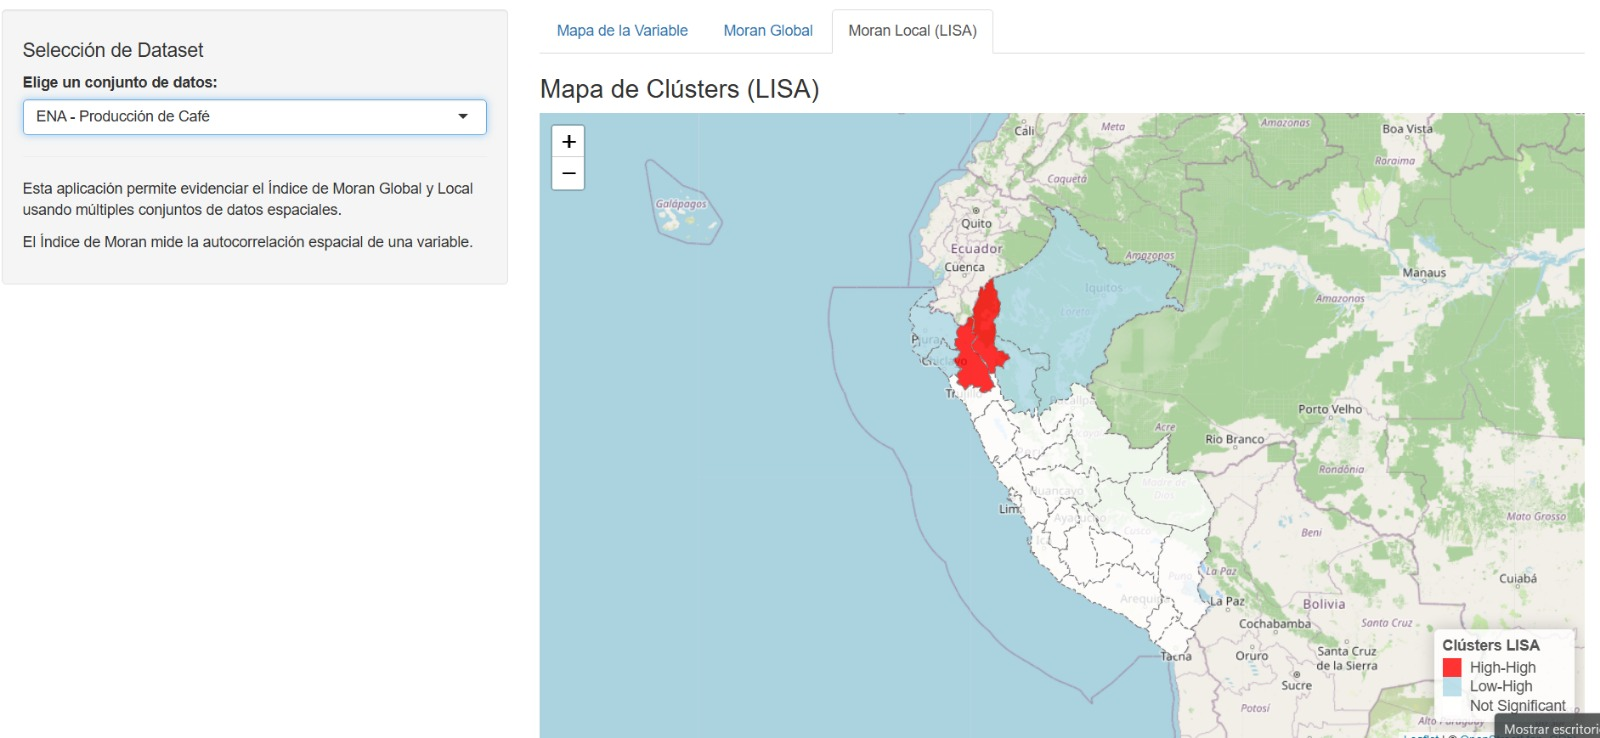
\includegraphics[width=0.95\textwidth]{mapa_lisa.jpeg}
    \caption{Mapeo de clústeres espaciales localmente significativos identificados por el algoritmo LISA (Local Indicators of Spatial Association).}
    \label{fig:mapa_lisa}
\end{figure}

Los resultados en el aplicativo categorizan los territorios peruanos en las siguientes zonas geo-económicas:
\begin{itemize}
    \item \textbf{Clústeres High-High (Alto-Alto):} Constituyen el núcleo productivo indiscutible. Son departamentos líderes en producción agraria fuertemente beneficiados por compartir fronteras con vecinos igualmente productivos. Evidencian \textit{hotspots} naturales para la economía agrícola.
    \item \textbf{Clústeres Low-Low (Bajo-Bajo):} Representan desiertos productivos relativos. Conforman extensas zonas (ej. regiones costeras desérticas para la papa, o zonas altitudinales gélidas para el café) donde la actividad agraria de dicho producto es económicamente nula o puramente de subsistencia.
    \item \textbf{Outliers (High-Low / Low-High):} Departamentos "rebeldes" que desafían la norma local. Ostentan producciones altísimas mientras todos sus vecinos decaen, o viceversa, apuntando a microclimas o fuertes inyecciones de inversión tecnológica encapsulada.
    \item \textbf{Espacios no significativos:} Zonas cuyo comportamiento oscila de manera aleatoria, imposibilitando la formación de un clúster sólido que soporte validación estadística rigurosa.
\end{itemize}

\section{Conclusiones y Recomendaciones de Política Agraria}
\begin{enumerate}
    \item \textbf{Madurez Computacional y Arquitectónica:} La ingeniería y limpieza de datos empleada (transición de 15 GB masivos a un formato binario consolidado) probó ser una habilidad crítica para la ciencia de datos. Permite trasladar simulaciones estadísticas de laboratorio a tableros de consumo web en tiempo real sin sacrificio de precisión.
    \item \textbf{Validación de Agrupamiento Natural:} La producción agrícola en el Perú no obedece a un proceso aleatorio. Tanto para la Papa como para el Café y el Maíz, la estadística rechaza fuertemente la hipótesis de aleatoriedad espacial completa. Existen ecosistemas departamentales fuertemente correlacionados que operan bajo lógicas conjuntas.
    \item \textbf{Decisiones Estatales Basadas en LISA:} Identificar clústeres locales \textit{High-High} provee evidencia científica innegable para la formulación de presupuestos y políticas públicas nacionales. Las iniciativas gubernamentales —como subsidios de fertilizantes, programas de irrigación, o asfaltado de vías de interconexión (corredores viales)— generarán un impacto y retorno de inversión multiplicador infinitamente mayor si se diseñan enfocadas en estas "macro-regiones o manchas calientes" identificadas por el Índice Local de Moran.
\end{enumerate}

\end{document}
